% =========================================================================== %

\begin{frame}[t,plain]
\titlepage
\end{frame}

% =========================================================================== %

\begin{frame}{Recap}
%
\begin{columns}[T]
\column{.5\linewidth}
\begin{itemize}
\item Sonderformen der Parameterliste
	\begin{itemize}
	\item Optionale Parameter
	\item Variadische Funktionen
	\item Keyword-Arguments
	\end{itemize}
\item Funktionen als Rückgabewert
	\begin{itemize}
	\item Rückgabe von Referenzen
	\item Funktionsgeneratoren
	\end{itemize}
\end{itemize}
%
\column{.5\linewidth}
\begin{itemize}
\item Lambdas
	\begin{itemize}
	\item Kurzschreibweise für Funktionen
	\item Oft als Parameter übergeben (\thus \texttt{sort})
	\end{itemize}
\item Rekursion
	\begin{itemize}
	\item Funktionen, die sich selbst aufrufen
	\item Lösung von selbstähnlichen Problemen
	\item \enquote{Boxen} mit eigenen Variablen gleichen Namens
	\end{itemize}
\end{itemize}

\end{columns}
%
\begin{center}
	\emph{Noch Fragen?}
\end{center}
%
\end{frame}

% =========================================================================== %
\begin{frame}[fragile]{Aus den Übungen}
%
\begin{codebox}[Lambdas als Suchschlüssel]
\begin{minted}[fontsize=\scriptsize, linenos]{python}
data = [(9, 1), (8, 2), (7, 3), (6, 4), (5, 5)]
print( sorted(data, key=lambda x: x[0]**2 + x[1]**2) )
\end{minted}
\end{codebox}
%
\begin{itemize}
\item Lambda: Abbildung \inPy{tuple} \thus Länge
\item Aufruf für jeden \inPy{tuple} in der \inPy{list data}
\item Sortierung dann aufsteigend nach Länge
\end{itemize}
%
\end{frame}

% =========================================================================== %

\begin{frame}[fragile]
%
\begin{codebox}[Binary Search \emph{mit} Rekursion]
\begin{minted}[fontsize=\scriptsize, linenos]{python}
def binarySearch (data, searchTerm) :
  size = len(data)
  
  if (size == 1) :
    if data[0] == searchTerm : return True
    else                     : return False
  else :
    midPoint = size // 2
    if   data[midPoint] == searchTerm : return True
    elif data[midPoint]  < searchTerm : return binarySearch(data[midPoint:], searchTerm)
    else                              : return binarySearch(data[:midPoint], searchTerm)

data = [1, 5, 6, 7, 8, 42, 96, 666, 1337, 2112]
searchTerm = 42

print("### binarySearch")
print(binarySearch(data, searchTerm) , end="\n\n")      # test for middle element
print(binarySearch(data, 1)          , end="\n\n")      # test for first element
print(binarySearch(data, 2112)       , end="\n\n")      # test for last element
print(binarySearch(data, 2)          , end="\n\n")      # test for not in list
\end{minted}
\end{codebox}
%
\end{frame}

% =========================================================================== %

\begin{frame}[fragile]
%
\begin{codebox}[Binary Search \emph{ohne} Rekursion]
\begin{minted}[fontsize=\scriptsize, linenos]{python}
def midSearch(data, searchTerm):
    first = 0
    last  = len(data)
    index = -1
    
    while(first <= last) and (index == -1):
        mid = (first+last) // 2
        if data[mid] == searchTerm:
            index = mid
        else:
            if searchTerm < data[mid]: last  = mid - 1
            else                     : first = mid + 1

    if index == -1: print("Element nicht in Liste enthalten")
    else          : return index

data = [1, 5, 6, 7, 8, 42, 96, 1337, 2112]
print(midSearch(data, 1337))
\end{minted}
\end{codebox}
%
\begin{flushright}
\scriptsize \emph{Danke an Michael Briehl für diesen Code}
\end{flushright}
%
\end{frame}

% =========================================================================== %

\begin{frame}[fragile]{Kapitel 7}
%
\begin{itemize}
\item Klassen als Datencontainer
\item Methoden
\item Magic Methods (\enquote{Dunders})
\end{itemize}
%
\end{frame}

% =========================================================================== %

\begin{frame}{Klassen}
%
\begin{itemize}
\item Grundidee: Computer \enquote{kennt} nur (Ganz)zahlen
\item Erst Interpretation dieser Zahlen gibt uns Texte, Bilder, Programme, ...
\item Beispiel: 98, 108, 117, 101
	\begin{itemize}
	\item ASCII-Codes der Zeichen \texttt{b, l, u, e}?
	\item oder Hausnummern der Adressen meiner ersten vier Freundinnen?
	\item \emph{Kontext} für Interpretation nötig
	\end{itemize}
\item Klassen: Datenobjekt, das Kontext gibt
	\begin{itemize}
	\item Sammlung mehrerer Werte
	\item Zugeordnete Interpretationsmethoden
	\end{itemize}
\item I.\;d.\;R. für \emph{ähnliche} Objekte \Thus Name \emph{Klassen}
\end{itemize}
%
\end{frame}

% =========================================================================== %

\begin{frame}[fragile]{Klassen in Python -- Datentypen}
%
\begin{columns}[T]
\column{.5\linewidth}
\begin{itemize}
\item Datentypen in Python sind bereits Beispiele für Klassen
	\begin{itemize}
	\item Beispiel: \inPy{list}s
	\item \enquote{Inhalt}: Listenelemente
	\item Zugeordnete Methoden: Sortieren, Umdrehen, Elemente Anhängen, ...
	\item \texttt{append} macht für einen \inPy{int} keinen Sinn!
	\end{itemize}
\item Klassen Entwickeln heißt: eigenen Datentypen erschaffen
\item Besteht im Inneren aus den bereits bekannten Typen
\end{itemize}
%
\column{.5\linewidth}
\begin{codebox}[Syntax: Klasse Anlegen]
\begin{minted}[fontsize=\scriptsize]{python}
class Klassenname :
    # Definitionen
\end{minted}
\end{codebox}

\begin{codebox}[Syntax: Instanz einer Klasse Anlegen]
\begin{minted}[fontsize=\scriptsize]{python}
newVar = Klassenname()
\end{minted}
\end{codebox}
\begin{itemize}
\item Hier viele Formen denkbar
\item Wichtigste Details Stück für Stück
\end{itemize}
\end{columns}
%
\end{frame}

% =========================================================================== %

\begin{frame}{Wer hatte es schwerer?}
%
\begin{center}
\scriptsize
\textbf{Stefans romantische Vergangenheit}
\rowcolors{1}{tabhighlight}{tabcontrast}
\begin{tabular}{c|ccp{.3\linewidth}p{.3\linewidth}}
	\textbf{Symbol} & \textbf{Name} & \textbf{Height} & \textbf{Upsides}                                 & \textbf{Downsides} \tabcrlf
	\texttt{exgf1}  & Steffie       & 1.65 m          & intelligent, beautiful, has a dog                & too attached to her mother, 
																																																				doesn't like meeting people \\
	\texttt{exgf2}  & Epsi          & 1.65 m          & very intelligent, beautiful, good taste in music & doesn't like coffee, doesn't like coding \\
	\texttt{exgf3}  & Katja         & 1.81 m          & intelligent, very beautiful, musician            & moody, cheated on me
\end{tabular}
\end{center}

\begin{center}
\scriptsize
\textbf{Charlottes gebrochene Herzen}
\rowcolors{1}{tabhighlight}{tabcontrast}
\begin{tabular}{c|ccp{.3\linewidth}p{.3\linewidth}}
	\textbf{Symbol} & \textbf{Name} & \textbf{Height} & \textbf{Upsides}                                 & \textbf{Downsides} \tabcrlf
	\texttt{exbf1}  & Sebastian     & 1.78 m          & intelligent, handsome, likes to listen           & obsessed with catching bugs, always late \\
	\texttt{exbf2}  & Reginald      & 1.84 m          & very intelligent, handsome, plays in a band      & flirty with everyone, complains a lot \\
	\texttt{exbf3}  & Sönke         & 1.81 m          & intelligent, quite handsome, cheerful nature     & superficial, racist
\end{tabular}
\end{center}
%
\end{frame}

% =========================================================================== %

\begin{frame}[fragile]{Klassen als reine Wert-Container}
%
\begin{codebox}[Syntax: Klasse mit \emph{Attributen}]
\begin{minted}[fontsize=\scriptsize]{python}
class Klassenname :
    Attribut1 = Wert1
    Attribut2 = Wert2
    ...
\end{minted}
\end{codebox}
%
\begin{codebox}[Syntax: Zugriff auf Attribute]
\begin{minted}[fontsize=\scriptsize]{python}
Instanz = Klassenname()

Instanz.Attribut1 = neuerWert
Klassenname.Attribut1 = neuerWert

Instanz.neuesAttribut = neuerWert
Klassenname.neuesAttribut = neuerWert
\end{minted}
\end{codebox}
%
\end{frame}

% =========================================================================== %

\begin{frame}[fragile]
%
\begin{tcbraster}[raster columns=2,
                  raster equal height,
                  nobeforeafter,
                  raster column skip=0.5cm]
\begin{codebox}[Beispiel: Attribute Ändern]
\begin{minted}[fontsize=\scriptsize, linenos]{python}
class cla :
    bar = "dead parrot"
    lst = [1]

foo = cla()

print("via foo:", foo.bar)
print("via cla:", cla.bar, end="\n\n")

cla.bar = "lumberjack"
print("via foo:", foo.bar)
print("via cla:", cla.bar, end="\n\n")

foo.bar = "hovercraft"
print("via foo:", foo.bar)
print("via cla:", cla.bar, end="\n\n")

foo.new = "eel"
print("via foo:", foo.new, end="\n\n")
# print("via cla:", cla.new)
\end{minted}
\end{codebox}
%
\begin{cmdbox}[Ausgabe: Attribute Ändern]
\begin{minted}[fontsize=\scriptsize]{text}
via foo: dead parrot
via cla: dead parrot

via foo: lumberjack
via cla: lumberjack

via foo: hovercraft
via cla: lumberjack

via cla: eel
\end{minted}
\end{cmdbox}
\end{tcbraster}
%
\end{frame}

% =========================================================================== %

\begin{frame}[fragile]
%
\begin{tcbraster}[raster columns=2,
                  raster equal height,
                  nobeforeafter,
                  raster column skip=0.5cm]
\begin{codebox}[Fortsetzung: Attribute Ändern]
\begin{minted}[fontsize=\scriptsize, linenos, firstnumber=20]{python}
# ...

foo.lst.append(2)
print("via foo:", foo.lst)
print("via cla:", cla.lst, end="\n\n")
\end{minted}
\end{codebox}
%
\begin{cmdbox}[Ausgabe: Fortsetzung]
\begin{minted}[fontsize=\scriptsize]{text}
...

via foo: [1, 2]
via cla: [1, 2]
\end{minted}
\end{cmdbox}
\end{tcbraster}
%
\end{frame}

% =========================================================================== %\\

\begin{frame}[fragile]
%
\begin{tcolorbox}[title=Speicherbild]
Bis Zeile 8 (nur Lese-Zugriffe):
\begin{center}
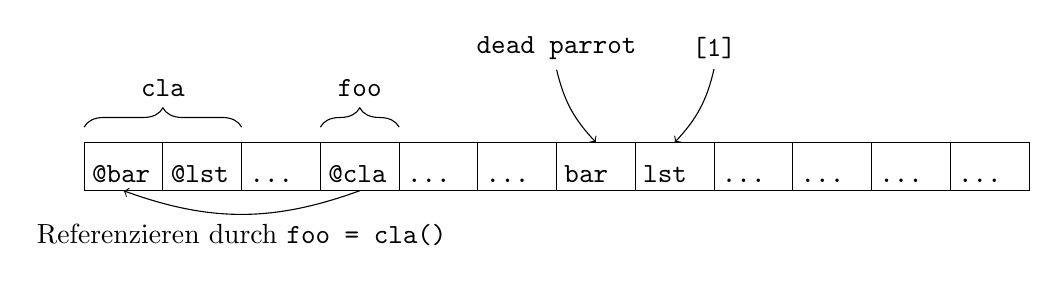
\begin{tikzpicture}
  [ 
    cell/.style={text width=8mm,
      text height=4mm, draw=black, inner sep=1mm},
    ld/.style={draw=blue,shorten >=2pt,->}
  ]
  \node  (a0) at ( 0,0) [cell] {\ttfamily @bar};
  \node  (a1) at ( 1,0) [cell] {\ttfamily @lst};
  \node  (a2) at ( 2,0) [cell] {\ttfamily ...};
  \node  (a3) at ( 3,0) [cell] {\ttfamily @cla};
  \node  (a4) at ( 4,0) [cell] {\ttfamily ...};
  \node  (a5) at ( 5,0) [cell] {\ttfamily ...};
  \node  (a6) at ( 6,0) [cell] {\ttfamily bar};
  \node  (a7) at ( 7,0) [cell] {\ttfamily lst};
  \node  (a8) at ( 8,0) [cell] {\ttfamily ...};
  \node  (a9) at ( 9,0) [cell] {\ttfamily ...};
  \node (a10) at (10,0) [cell] {\ttfamily ...};
  \node (a11) at (11,0) [cell] {\ttfamily ...};
  
  \draw [decorate, decoration={brace,amplitude=7pt}, xshift=-0pt, yshift=0pt]
  		(-0.5, 0.5) -- ( 1.5, 0.5) node (x) [midway, yshift=+0.5cm] 
		(braceFuncDerivative) {\texttt{cla}};
	
  \draw [decorate, decoration={brace,amplitude=7pt}, xshift=-0pt, yshift=0pt]
  		( 2.5, 0.5) -- ( 3.5, 0.5) node (y) [midway, yshift=+0.5cm] 
		(braceFuncDerivative) {\texttt{foo}};
	
	\draw [->, bend left=20]
		(a3.south) to node 
		[below] {Referenzieren durch \texttt{foo = cla()}} 
		(a0.south);
		
	\node (t6) at (5.5,+1.5) {\texttt{dead parrot}};
	\node (t7) at (7.5,+1.5) {\texttt{[1]}};
	
	\draw [->, bend right=15] (t6.south) to node [below] {} (a6.north);
	\draw [->, bend left =15] (t7.south) to node [below] {} (a7.north);
\end{tikzpicture}
\end{center}
\texttt{foo} enthält nur eine Referenz auf \texttt{cla}; dieses Symbol wiederum referenziert \texttt{bar} und \texttt{lst}.
\end{tcolorbox}
%
\end{frame}

% =========================================================================== %\\

\begin{frame}[fragile]
%
\begin{tcolorbox}[title=Speicherbild]
Zeile 10: \inPy{cla.bar = "lumberjack"}
\begin{center}
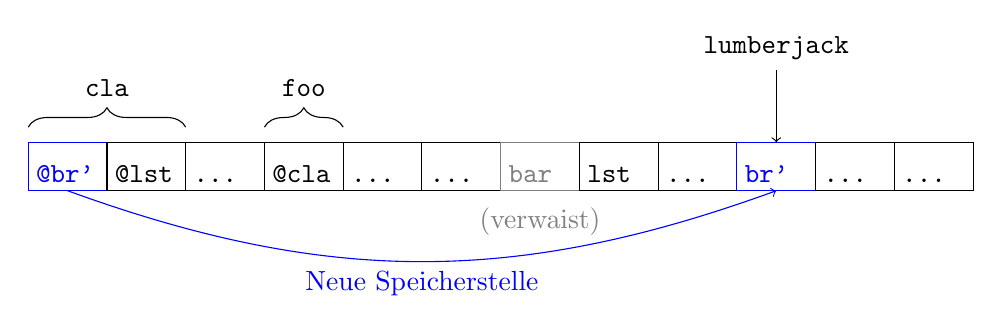
\begin{tikzpicture}
  [ 
    cell/.style={text width=8mm,
      text height=4mm, draw=black, inner sep=1mm},
    ld/.style={draw=blue,shorten >=2pt,->}
  ]
  \node  (a0) at ( 0,0) [cell, blue] {\ttfamily @br'};
  \node  (a1) at ( 1,0) [cell] {\ttfamily @lst};
  \node  (a2) at ( 2,0) [cell] {\ttfamily ...};
  \node  (a3) at ( 3,0) [cell] {\ttfamily @cla};
  \node  (a4) at ( 4,0) [cell] {\ttfamily ...};
  \node  (a5) at ( 5,0) [cell] {\ttfamily ...};
  \node  (a6) at ( 6,0) [cell, gray] {\ttfamily bar};
  \node  (a7) at ( 7,0) [cell] {\ttfamily lst};
  \node  (a8) at ( 8,0) [cell] {\ttfamily ...};
  \node  (a9) at ( 9,0) [cell, blue] {\ttfamily br'};
  \node (a10) at (10,0) [cell] {\ttfamily ...};
  \node (a11) at (11,0) [cell] {\ttfamily ...};
  
  \draw [decorate, decoration={brace,amplitude=7pt}, xshift=-0pt, yshift=0pt]
  		(-0.5, 0.5) -- ( 1.5, 0.5) node (x) [midway, yshift=+0.5cm] 
		(braceFuncDerivative) {\texttt{cla}};
	
  \draw [decorate, decoration={brace,amplitude=7pt}, xshift=-0pt, yshift=0pt]
  		( 2.5, 0.5) -- ( 3.5, 0.5) node (y) [midway, yshift=+0.5cm] 
		(braceFuncDerivative) {\texttt{foo}};
	
	\draw [->, bend right=20, blue]
		(a0.south) to node 
		[below] {Neue Speicherstelle} 
		(a9.south);
	
	\node (t6) at (6,-0.7) {\color{gray}(verwaist)};
	
	\node (t9) at (9,+1.5) {\texttt{lumberjack}};
	\draw [->] (t9.south) to node [below] {} (a9.north);
\end{tikzpicture}
\end{center}
Änderungen an \texttt{cls} beeinflussen auch \texttt{foo}, da dieses nur eine Referenz auf \texttt{cla} enthält.\\
Da \texttt{bar} ein String und damit immutable ist, erzeugen Änderungen hieran eine neue Speicherstelle. Die alte Speicherstelle verfällt.
\end{tcolorbox}
%
\end{frame}

% =========================================================================== %\\

\begin{frame}[fragile]
%
\begin{tcolorbox}[title=Speicherbild]
Zeile 14: \inPy{foo.bar = "hovercraft"}\\
Zeile 18: \inPy{foo.new = "eel"}
\begin{center}
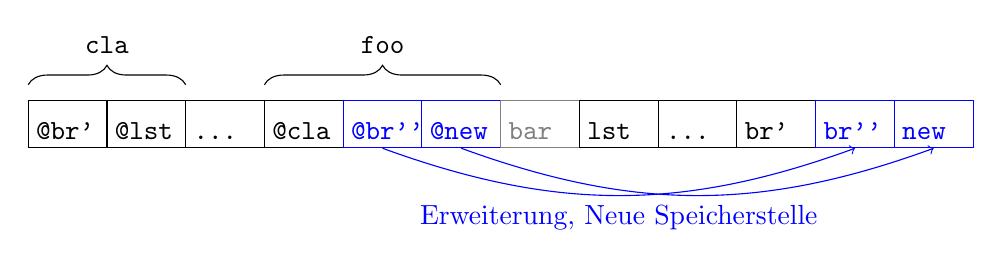
\begin{tikzpicture}
  [ 
    cell/.style={text width=8mm,
      text height=4mm, draw=black, inner sep=1mm},
    ld/.style={draw=blue,shorten >=2pt,->}
  ]
  \node  (a0) at ( 0,0) [cell] {\ttfamily @br'};
  \node  (a1) at ( 1,0) [cell] {\ttfamily @lst};
  \node  (a2) at ( 2,0) [cell] {\ttfamily ...};
  \node  (a3) at ( 3,0) [cell] {\ttfamily @cla};
  \node  (a4) at ( 4,0) [cell, blue] {\ttfamily @br''};
  \node  (a5) at ( 5,0) [cell, blue] {\ttfamily @new};
  \node  (a6) at ( 6,0) [cell, gray] {\ttfamily bar};
  \node  (a7) at ( 7,0) [cell] {\ttfamily lst};
  \node  (a8) at ( 8,0) [cell] {\ttfamily ...};
  \node  (a9) at ( 9,0) [cell] {\ttfamily br'};
  \node (a10) at (10,0) [cell, blue] {\ttfamily br''};
  \node (a11) at (11,0) [cell, blue] {\ttfamily new};
  
  \draw [decorate, decoration={brace,amplitude=7pt}, xshift=-0pt, yshift=0pt]
  		(-0.5, 0.5) -- ( 1.5, 0.5) node (x) [midway, yshift=+0.5cm] 
		(braceFuncDerivative) {\texttt{cla}};
	
  \draw [decorate, decoration={brace,amplitude=7pt}, xshift=-0pt, yshift=0pt]
  		( 2.5, 0.5) -- ( 5.5, 0.5) node (y) [midway, yshift=+0.5cm] 
		(braceFuncDerivative) {\texttt{foo}};
	
	\draw [->, bend right=20, blue]
		(a4.south) to node 
		[below] {Erweiterung, Neue Speicherstelle} 
		(a10.south);
	\draw [->, bend right=20, blue]
		(a5.south) to node 
		[below] {}
		(a11.south);
\end{tikzpicture}
\end{center}
An \texttt{foo} werden Ergänzungen durchgeführt, die die Vorgaben von \texttt{cla} ersetzen. Neue Speicherstellen werden angelegt. \\
Abgesehen von den Ergänzungen gilt weiter die Struktur von \texttt{cla}! Zugriffe auf \texttt{foo.lst} gehen weiter über \texttt{cla}.\\
\texttt{lst} ist \emph{mutable}, daher wird \emph{keine neue Speicherstelle} angelegt.
\end{tcolorbox}
%
\end{frame}

% =========================================================================== %\\

\begin{frame}
%
\begin{hintbox}[Klassenattribute und Instanz-Attribute]
Wir unterscheiden also Attribute, die alle Instanzen der Klasse \emph{gemeinsam} haben, und solche, die spezifisch für die Instanz sind.

Im Beispiel der ExfreundInnen: Klassenattribut könnte ein \emph{gemeinsamer} Wertmaßstab sein; Instanz-Attribute sind die Eigenschaften der ExpartnerInnen

Klassenattribute werden \emph{in der Klasse} festgelegt. Instanz-Attribute werden erst an den Instanzen definiert.
\end{hintbox}
%
\end{frame}

% =========================================================================== %

\begin{frame}[fragile]
%
\begin{codebox}[Beispiel: Klassen- und Instanz-Attribute]
\begin{minted}[linenos, fontsize=\scriptsize]{python}
class Expartner :
    traits = {
        "good taste in music"         :   2, "beautiful"                   :   3,
        "handsome"                    :   3, "intelligent"                 :   5,
        "very beautiful"              :   5, "very handsome"               :   5,
        "very intelligent"            :  10, "doesn't like coding"         : - 4,
        "doesn't like meeting people" : - 4, "complains a lot"             : - 8,
        "cheated on me"               : -20, "racist"                      : -30
    }

exgf2 = Expartner()
exgf2.name      = "Epsi"
exgf2.height    = 1.65
exgf2.upsides   = {"very intelligent", "beautiful", "good taste in music"}
exgf2.downsides = {"doesn't like coffee", "doesn't like coding"}

exbf2 = Expartner()
exbf2.name      = "Reginald"
exbf2.height    = 1.84
exbf2.upsides   = {"very intelligent", "handsome", "plays in a band"}
exbf2.downsides = {"flirty with everyone", "complains a lot"}
\end{minted}
\end{codebox}
%
\end{frame}

% =========================================================================== %

\begin{frame}[fragile]{Klassen-Methoden}
%
\begin{columns}[T]
\column{.5\linewidth}
\begin{itemize}
\item Methode: Funktion, die auf eine Instanz angewandt werden soll
\item Definition \emph{in der Klasse}
\item Verpflichtender erster Parameter: \inPy{self}
	\begin{itemize}
	\item Enthält Bezug zur Instanz, auf die die Methode angewandt wird
	\item[\Thus] Zugriff auf Klassen- und Instanzattribute über \inPy{self}
	\item Wird automatisch beim Methoden-Aufruf übergeben
	\item Name ist Konvention, nicht Verpflichtung
	\end{itemize}
\item Jede Klasse verwaltet eigene Namenslisten
\end{itemize}
%
\column{.5\linewidth}
\begin{codebox}[Syntax: Definition Klassenmethode]
\begin{minted}[fontsize=\scriptsize]{python}
class Klassenname :
    ...
    def Methode(self, ...) :
       Code
    ...
\end{minted}
\end{codebox}
%
\begin{codebox}[Syntax: Aufruf Klassenmethode]
\begin{minted}[fontsize=\scriptsize]{python}
Instanz = Klassenname()
Instanz.Methode(...)
\end{minted}
\end{codebox}
%
\begin{itemize}
\item[\Thus] zwei verschiedene Klassen dürfen je eine Methode mit gleichem Namen haben
\end{itemize}
\end{columns}
%
\end{frame}

% =========================================================================== %

\begin{frame}[fragile]
%
\begin{codebox}[Beispiel: Klassenmethoden]
\begin{minted}[linenos, fontsize=\scriptsize]{python}
class Expartner :
    traits = { ... }   # wie zuvor
    
    def rating(self) :
        reVal = 0
        for trait in self.upsides :
            if trait in self.traits : reVal += self.traits[trait]
            else                    : reVal += +1
        for trait in self.downsides :
            if trait in self.traits : reVal += self.traits[trait]
            else                    : reVal += -1
        return reVal
   
    def areThey(self, trait) :
        return (trait in self.upsides) or (trait in self.downsides)

# exgf2, exbf2 wie zuvor

print( exgf2.arethey("very intelligent") )   # Ausgabe: True
print( exbf2.rating() )                      # Ausgabe: 5
\end{minted}
\end{codebox}
%
\end{frame}


% =========================================================================== %

\begin{frame}{Magic Methods (\enquote{Dunders})}
%
\begin{itemize}
\item Funktionsaufrufe manchmal umständlich, oder schlechter lesbar.
	\begin{itemize}
	\item Vergleiche: \inPy{x + y} mit \inPy{x.add(y)}
	\end{itemize}
\item Für häufig auftretende Operationen daher: eigener Mechanismus
\item Funktionen, die automatisch aufgerufen werden
	\begin{itemize}
	\item Initialisieren: \inPy{__init__}
	\item Rechenoperationen: \inPy{__add__}, \inPy{__sub__}, \inPy{__mul__}, \inPy{__matmul__}, \inPy{__truediv__}, \inPy{__floordiv__}
	\item Vergleiche: \inPy{__eq__}, \inPy{__ne__}, \inPy{__gt__}, \inPy{__ge__}, \inPy{__lt__}, \inPy{__le__}
	\item Stringdarstellung: \inPy{__str__} und \inPy{__repr__}
	\item Gebrauch als Funktion: \inPy{__call__}
	\end{itemize}
\item \emph{Double Underscore} \Thus \enquote{Dunders}
\end{itemize}
%
\end{frame}

% =========================================================================== %

\begin{frame}[fragile]
%
\begin{columns}[T]
\column{.5\linewidth}
\begin{Large}
	{\inPy{__init__} -- Konstruktor}
\end{Large}
\vspace{6pt}
%
\begin{itemize}
\item Wird aufgerufen, sobald Instanz angelegt wird
\item Nach \inPy{self}: freie Form
\item Üblicherweise: Eintragen von Standardwerten
\end{itemize}
%
\column{.5\linewidth}
\begin{codebox}[Syntax: \texttt{\_\_init\_\_}]
\begin{minted}[fontsize=\scriptsize]{python}
class Klassenname :
    # Klassenattribute
    
    def __init__ (self, ...) :
        ...
\end{minted}
\end{codebox}
%
\begin{codebox}[Syntax: Aufruf \texttt{\_\_init\_\_}]
\begin{minted}[fontsize=\scriptsize]{python}
Instanz = Klassenname(...)
\end{minted}
\end{codebox}
\end{columns}
%
\end{frame}

% =========================================================================== %

\begin{frame}[fragile]
%
\begin{codebox}[Beispiel: \texttt{\_\_init\_\_}]
\begin{minted}[linenos, fontsize=\scriptsize]{python}
class Expartner :
    # Klassenattribute ...
    
    def __init__(self, name = None, height = None,
                 upsides = {}, downsides = {}) :
        if height < 0 :
            raise Exception("Your Ex cannot be less than 0.0m tall")
        
        self.name      = name
        self.height    = height
        self.upsides   = upsides
        self.downsides = downsides
    
perfect = Expartner("Arista" , 1.70, 
              {"very intelligent", "very beautiful", "good taste in music"}
          )
\end{minted}
\end{codebox}
%
\end{frame}

% =========================================================================== %

\begin{frame}[fragile]
%
\begin{columns}[T]
\column{.5\linewidth}
\begin{Large}
	{\inPy{__str__} und \inPy{__repr__} -- Textdarstellung}
\end{Large}
\vspace{6pt}
%
\begin{itemize}
\item Beide Funktionen: Text, der die Klasseninstanz repräsentiert
\item \inPy{__str__}
	\begin{itemize}
	\item \enquote{schöne Form}, für den End-User
	\item Automatisch Aufgerufen über \inPy{str(Instanz)}
	\item \inPy{print} ruft automatisch \inPy{str} für jedes Argument auf
	\end{itemize}
\item \inPy{__repr__}
	\begin{itemize}
	\item knappe Form, häufig zum Debuggen 
	\item Automatisch Aufgerufen über \inPy{repr(Instanz)}
	\end{itemize}
\item beide: Keine Parameter
\end{itemize}
%
\column{.5\linewidth}
\begin{codebox}[Syntax: \texttt{\_\_str\_\_} und \texttt{\_\_repr\_\_}]
\begin{minted}[fontsize=\scriptsize]{python}
class Klassenname :
    # Klassenattribute
    
    def __repr__ (self) :
        return someString
    
    def __str__ (self) :
        return someString
\end{minted}
\end{codebox}
%
\begin{codebox}[Syntax: Aufruf \texttt{\_\_str\_\_} und \texttt{\_\_repr\_\_}]
\begin{minted}[fontsize=\scriptsize]{python}
Instanz = Klassenname()

print(Instanz)         # beide
print(str(Instanz))    # gleich
pritn(repr(Instanz))
\end{minted}
\end{codebox}
\end{columns}
%
\end{frame}

% =========================================================================== %

\begin{frame}[fragile]
%
\begin{columns}[T]
\column{.5\linewidth}
\begin{Large}
	{\inPy{__call__} -- Aufruf als Funktion}
\end{Large}
\vspace{6pt}
%
\begin{itemize}
\item Idee: Gebrauche Instanz wie eine Funktion
\item Beispielsweise für Spiel, das viele Parameter verwaltet:
	\begin{minted}{python}
	partie = Spiel()
	partie.Spielerzahl = 2
	partie.Zeitlimit = 30
	...
	partie()
	\end{minted}
\item Beliebige Art und Anzahl von Parametern
\end{itemize}
%
\column{.5\linewidth}
\begin{codebox}[Syntax: \texttt{\_\_call\_\_}]
\begin{minted}[fontsize=\scriptsize]{python}
class Klassenname :
    # Klassenattribute
    
    def __call__ (self, ...) :
        ...

\end{minted}
\end{codebox}
%
\begin{codebox}[Syntax: Aufruf \texttt{\_\_call\_\_}]
\begin{minted}[fontsize=\scriptsize]{python}
Instanz = Klassenname()

Instanz(...)
\end{minted}
\end{codebox}
\end{columns}
%
\end{frame}

% =========================================================================== %

\begin{frame}[fragile]
%
\begin{codebox}[Beispiel: Aufruf als Funktion]
\begin{minted}[linenos, fontsize=\scriptsize]{python}
class Expartner :
    # wie oben
    
    def __call__(self) :
        print("You shouldn't call your Ex'es. Leave the past behind.")

ex = Expartner("Sandra", 1.70)
ex()
\end{minted}
\end{codebox}
%
\end{frame}